% !TeX document-id = {04abaeb2-125e-4994-ab3e-b16c105b617d}
% !TeX program = xelatex ?me -synctex=0 -interaction=nonstopmode -aux-directory=../tex_aux -output-directory=./release
% !TeX program = xelatex

\documentclass[12pt]{article}

\usepackage{lineno,changepage,lipsum}
\usepackage[colorlinks=true,urlcolor=blue]{hyperref}
\usepackage{fontspec}
\usepackage{xeCJK}
\usepackage{tabularx}
\setCJKfamilyfont{chanto}{AozoraMinchoRegular.ttf}
\setCJKfamilyfont{tegaki}{Mushin.otf}
\usepackage[CJK,overlap]{ruby}
\usepackage{hhline}
\usepackage{multirow,array,amssymb}
\usepackage[croatian]{babel}
\usepackage{soul}
\usepackage[usenames, dvipsnames]{color}
\usepackage{wrapfig,booktabs}
\renewcommand{\rubysep}{0.1ex}
\renewcommand{\rubysize}{0.75}
\usepackage[margin=50pt]{geometry}
\modulolinenumbers[2]

\usepackage{pifont}
\newcommand{\cmark}{\ding{51}}%
\newcommand{\xmark}{\ding{55}}%

\definecolor{faded}{RGB}{100, 100, 100}

\renewcommand{\arraystretch}{1.2}

%\ruby{}{}
%$($\href{URL}{text}$)$

\newcommand{\furigana}[2]{\ruby{#1}{#2}}
\newcommand{\tegaki}[1]{
	\CJKfamily{tegaki}\CJKnospace
	#1
	\CJKfamily{chanto}\CJKnospace
}

\newcommand{\dai}[1]{
	\vspace{20pt}
	\large
	\noindent\textbf{#1}
	\normalsize
	\vspace{20pt}
}

\newcommand{\fukudai}[1]{
	\vspace{10pt}
	\noindent\textbf{#1}
	\vspace{10pt}
}

\newenvironment{bunshou}{
	\vspace{10pt}
	\begin{adjustwidth}{1cm}{3cm}
	\begin{linenumbers}
}{
	\end{linenumbers}
	\end{adjustwidth}
}

\newenvironment{reibun}{
	\vspace{10pt}
	\begin{tabular}{l l}
}{
	\end{tabular}
	\vspace{10pt}
}
\newcommand{\rei}[2]{
	#1&\textit{#2}\\
}
\newcommand{\reinagai}[2]{
	\multicolumn{2}{l}{#1}\\
	\multicolumn{2}{l}{\hspace{10pt}\textit{#2}}\\
}

\newenvironment{mondai}[1]{
	\vspace{10pt}
	#1
	
	\begin{enumerate}
		\itemsep-5pt
	}{
	\end{enumerate}
	\vspace{10pt}
}

\newenvironment{hyou}{
	\begin{itemize}
		\itemsep-5pt
	}{
	\end{itemize}
	\vspace{10pt}
}

\date{\today}

\CJKfamily{chanto}\CJKnospace

\usepackage{tikz}
\newcommand{\en}[1]{
	\begin{tikzpicture}[baseline=(C.base)]
	\node[draw,circle,inner sep=1pt](C){#1};
	\end{tikzpicture}
}

\author{Tomislav Mamić}
\begin{document}
	\dai{Vremenske imenice}
	
	\fukudai{Teorija - priložne imenice}
	
	Ovu smo temu okrznuli na početnim radionicama kad smo učili o priložnim oznakama vremena. Tada smo rekli da u japanskom jeziku postoje imenice koje imaju gramatičku funkciju - koje određuju odnos između svog opisa i ostatka rečenice, i tu smo stali. Sada, znajući ponešto o opisnim rečenicama, možemo u detalje proučiti ovaj vrlo važan gramatički mehanizam. Uzmimo za primjer neke česte vremenske imenice:
	
	\begin{reibun}
		\rei{とき}{vrijeme}
		\rei{ころ}{vrijeme, period, razdoblje}
		\rei{しゅんかん}{trenutak}
	\end{reibun}

	\noindent
	Nabrojane imenice imaju konkretno značenje - rečenici mogu dodati sadržaj:
	
	\begin{reibun}
		\rei{その ときが 来た。}{Došlo je to vrijeme.}
	\end{reibun}

	\noindent
	Vrlo je često neprirodno prevoditi ili uopće razmatrati konkretno značenje priložnih imenica:
	
	\begin{reibun}
		\reinagai{猫を見た ときの 花子ちゃんの えがおは わすれません。}{Neću zaboraviti osmjeh koji je Hanako imala na licu kad je vidjela mačku.}
		\reinagai{日本に すんでいた ころ、まいにち ラーメンを 食べていた。}{Kad sam živio u Japanu, svaki dan sam jeo r\={a}men.}
	\end{reibun}

	\noindent
	Uočimo kako u rečenicama iznad nismo preveli ni とき ni ころ, već smo njihove opise u hrvatskom preveli kao zavisne rečenice koje opisuju vrijeme glavne. Ovo je bitna osobina svih priložnih imenica.
	
	\fukudai{Opisivanje \textit{kad} se nešto dogodilo}
	
	Već znamo reći da se nešto dogodilo \textit{jučer} ili \textit{prošle godine}. Koristeći vremenske imenice možemo sastaviti složene rečenice s vrlo bogatim priložnim oznakama vremena. Uz dvije ranije spomenute rečenice, pogledajmo primjere:
	
	\begin{reibun}
		\reinagai{こどもの ころ、川の そばで あそんでいた。}{Kao dijete sam se često igrao u blizini rijeke.}
		\reinagai{みちを わたる とき、くるまに きを つけてください。}{Kad prelaziš cestu, pazi na aute.}
		\reinagai{\parbox{480pt}{かれの かおに むかって とんで くる 猫に きが ついた しゅんかん、たけしは 「これは まちがい だった」と おもった。}}{\parbox{480pt}{U trenu kad je spazio mačku koja leti prema njegovom licu, Takeši je pomislio kako je ovo bilo pogreška.}}
		\reinagai{かれに であった あの日は いまも よく おぼえている。}{I sad se dobro sjećam onog dana kad sam ga upoznao.}
	\end{reibun}

	Uočimo kako je prijevod ovih priložnih oznaka vremena vrlo proizvoljan (npr. \textit{kao dijete sam} umjesto \textit{kad sam bio dijete}) - bitno je prenijeti značenje u duhu jezika, a ne gramatičku strukturu.

	\fukudai{Opisivanje intervala u kojem se nešto dogodilo}
	
	Koristeći imenice あいだ i うち (obje u rječniku imaju preko nekoliko različitih prijevoda) možemo izraziti značenje koje u hrvatskom postižemo riječju \textit{dok}:
	
	\begin{reibun}
		\reinagai{ともだちを まっている あいだ(に)、本を よんでいた。}{Dok sam čekao prijatelja, čitao sam knjigu.}
		\reinagai{ははが 食べている うちに、たけしくんは いえを でた。}{Dok je majka jela, Takeši je izišao iz kuće.}
		\reinagai{ちかい うちに\footnotemark[1] あらしが 来る。}{Uskoro dolazi oluja.}
	\end{reibun}

	U primjerima s glagolima iznad, zgodno je uočiti da predikati zavisnih rečenica izriču trenutno stanje (\textasciitilde ている) i da su u potvrdnom, neprošlom obliku. Imenice あいだ i うち u ovoj upotrebi \textbf{nikad nećemo opisivati} predikatom u prošlom vremenu. Negiramo li predikat, značenje se prigodno mijenja:
	
	\begin{reibun}
		\reinagai{ははが 見ていないうちに、たけしくんは いえを でた。}{Dok majka nije gledala, Takeši je izišao iz kuće.}
		\reinagai{先生が まだ 来ていない あいだに まどから きょうしつに はいった。}{Dok učitelj još nije došao, ušao sam u učionicu kroz prozor.}
	\end{reibun}

	\noindent
	Ukoliko negirani predikat ne izriče stanje, dobivamo nešto drugačiji smisao:
	
	\begin{reibun}
		\reinagai{先生が 来ない うちに まどから きょうしつに はいる。}{Ući ću u učionicu kroz prozor prije nego učitelj dođe.}
		\reinagai{花子ちゃんは さくらの花が ちらない うちに 日本に もどりたい。}{Hanako se želi vratiti u Japan prije nego trešnje ocvatu.}
	\end{reibun}

	\footnotetext[1]{Izraz ちかいうちに kao \textit{uskoro, ubrzo} je čest i koristan. Ovdje nije uobičajeno reći あいだ.}
	
	Gledajući brojeve na slici u nastavku, možemo im pridružiti sljedeće događaje:
	
	\begin{hyou}
		\item \en{1} さくらの花が さく
		\item \en{2} さくらの花が ちる
		\item \en{3} さくらの花が さいている うちに
		\item \en{4} さくらの花が ちらない うちに
	\end{hyou}
	
	\begin{figure}[h]
		\centering
		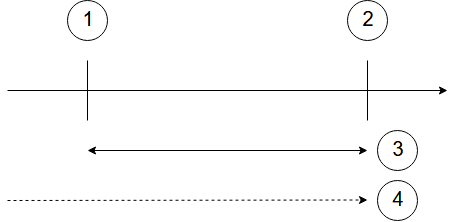
\includegraphics[width=200pt]{img/vrem_1}
		\caption{Trenuci na koje upućuju upotrebe \textasciitilde~うちに.}
	\end{figure}

	\fukudai{Vježba}
	
	\begin{mondai}{Prevedite na hrvatski:}
		\item きょねん 日本に 行った ときは さむかった。
		\item こどもの ころ、にんじんが きらいだった。
		\item ねずみを 見た しゅんかん、猫は 目を さました。\\(目を さます - izraz, \textit{probuditi se})
		\item こどもが ねている あいだは しずかに してください。\\(しずかに する - izraz, \textit{biti tiho})
		\item 花子ちゃんが いえに いない とき、猫は さびしく なる。\\(さびしい - \textit{usamljen})
		\item 花子ちゃんが いえに いない あいだに 猫は まくらの うえで ねていた。\\(まくら - \textit{jastuk})
		\item ごはんが さめない うちに たべてください。\\(さめる - \textit{ohladiti se})
	\end{mondai}

	\begin{mondai}{Prevedite na japanski:}
		\item Sljedeći put kad odeš u Japan, kupi mi neki suvenir.\\korisno: こんど - \textit{sljedeći put}, おみやげ - \textit{suvenir}
		\item Kad sam bio dijete sam mrzio mrkve, ali sada ih volim.
		\item Čim je čuo Hanako, Takeši je ušao u kutiju.\\korisno: とたん - slično kao しゅんかん, ali se često prevodi kao \textit{čim}
		\item Dok se Takeši igrao, Hanako je napisala domaću zadaću.\\korisno: しゅくだい domaća zadaća
		\item Želim se vratiti kući prije nego počne kiša.
	\end{mondai}

\end{document}